\subsection{بخش پ}
در این بخض دو نوع روش هدایت بررسی شده است. روش اول تنها از روش هدایت تناسبی خالص استفاده شده است و روش دوم از روش هدایت تناسبی خالص و غیرخطی. نتایج در ادامه آورده شده است.
\begin{figure}[H]
    \label{fig:q2_1}
	\centering
	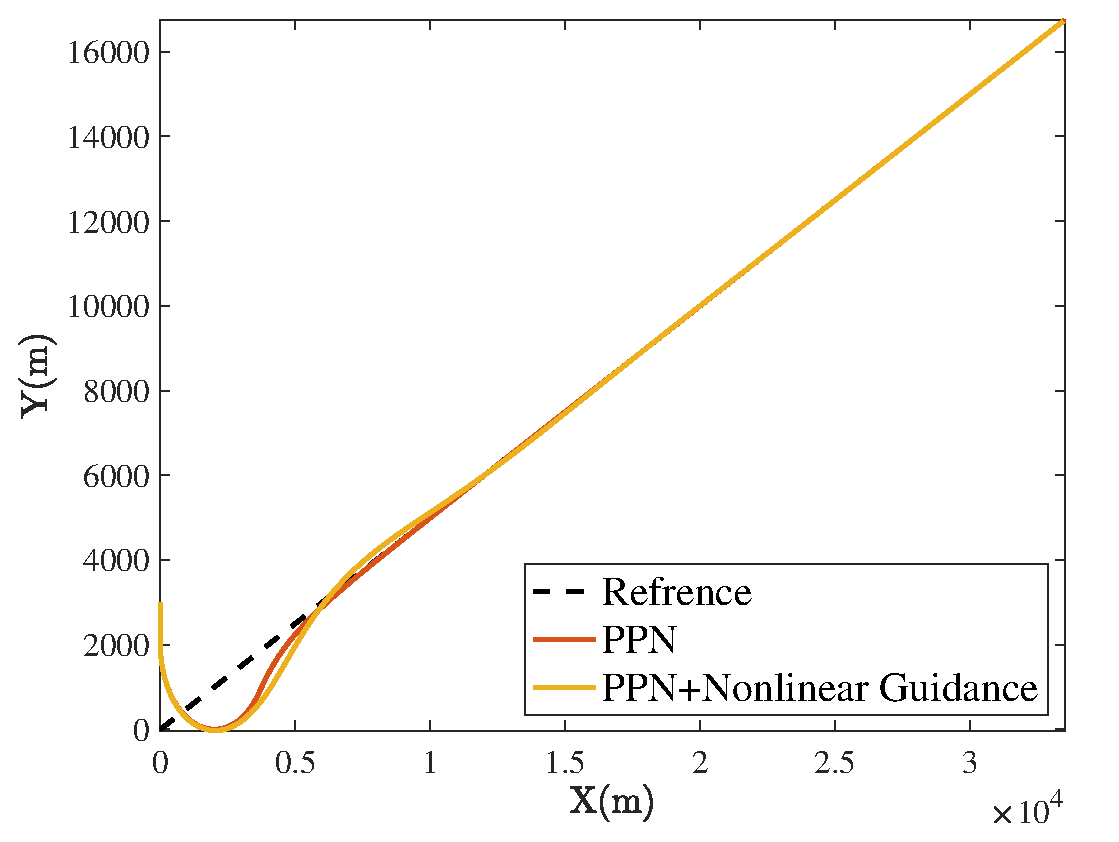
\includegraphics[width=.75\linewidth]{../Figure/Q2/c/xy}
    \caption{موقعیت پهپاد در صفحه X-Y   در روش هدایت تناسبی خالص و غیرخطی}
\end{figure}

\begin{figure}[H]
    \label{fig:q2_1}
	\centering
	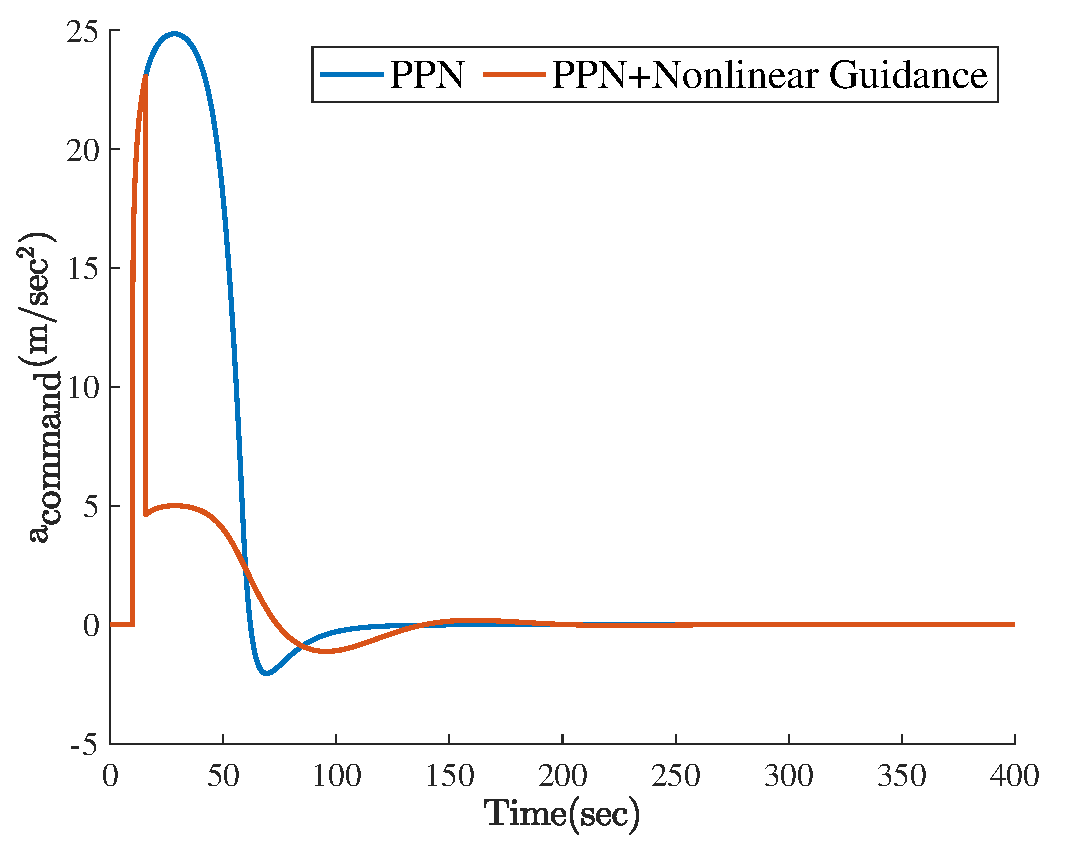
\includegraphics[width=.75\linewidth]{../Figure/Q2/c/acc}
    \caption{فرمان هدایت به‌صورت تابعی از زمان در روش هدایت تناسبی خالص و غیرخطی}
\end{figure}
